\documentclass [a4paper,12pt]{paper}

\usepackage{mycommands}


\title{Lecture 17: The spherical Earth}
\author{David Al-Attar \\ Michaelmas Term, \the\year}

\begin{document}

\maketitle

\section*{Outline and motivation}

In this lecture we apply ray theory to explain how quantitative properties of earthquakes and the Earth's internal structure can be determined from observations of seismic waves.
 Most of the methods and results we describe are more than seventy years old, are not representative of current research in seismology. They are, nonetheless, still of great value, 
 and later developments in the field have been built on these foundations. Indeed, it is really quite remarkable that most of the knowledge about the Earth and earthquakes contained 
 within this lecture was determined at a time before digital seismometers and electronic computers.

\section*{Hypocentre location using high-frequency waves}


\begin{figure}[h]
\centering
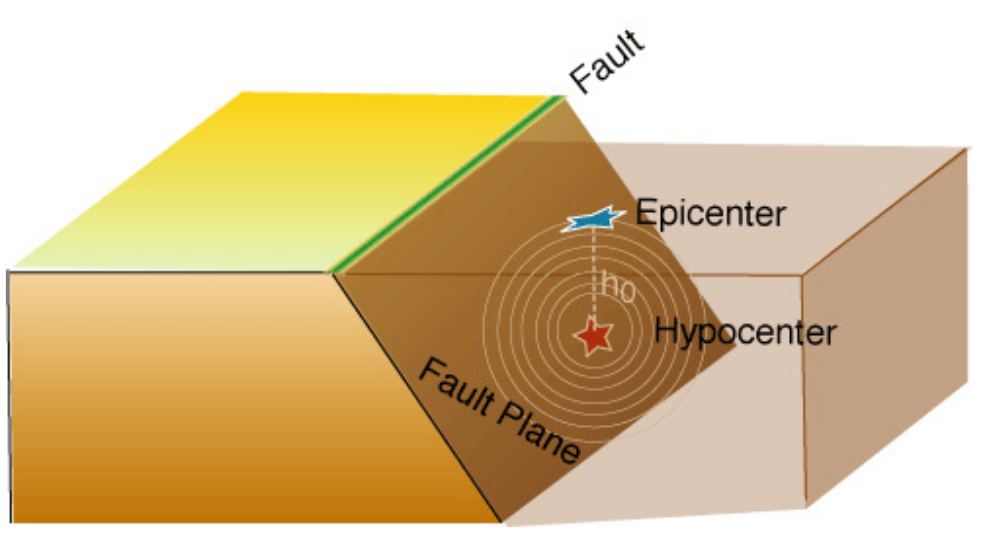
\includegraphics[width=0.8\textwidth]{figures/L6F1.png}
\caption{A diagram showing an idealised planar fault. The hypocentre is the point on
the fault where rupture initiates, while the epicentre is simply the projection of
this point onto the Earth’s surface. It is the hypocentre location that can be
estimated by looking at the arrival times of high-frequency seismic waves recorded
on seismometers.}
\label{fig:fig1}
\end{figure}

Natural earthquakes occur due to rupture on faults within the Earth, and the point on the fault at which this rupture initiates is known as the earthquake's hypocentre. Fracture 
mechanics tells us that the speed of rupture propagation on the fault must be less than the fastest elastic wave speed of the medium (e.g. the p-wave speed in isotropic bodies), 
and it follows that the first waves to be recorded at distant seismometers are generated at the hypocentre. Using the recorded arrival times of the first seismic waves at a large 
number of seismometers, it is possible to estimate the hypocentre location.

We shall focus on the case of an earthquake recorded at a large number of seismometers around the globe, and assume that the Earth's elastic properties are isotropic, which is a 
reasonable first-approximation. On a global scale, seismic waves can be recorded at frequencies up to about 2Hz. The reason for this upper frequency limit is two-fold: (i) earthquakes 
generate energy at a whole range of frequencies, but the spectrum tends to be biased towards lower frequencies, and (ii) attenuation mechanisms for seismic waves (which we have not 
discussed) act more strongly at higher frequencies, and so higher frequency components of the wavefield are removed more quickly as they propagate through the Earth. At the highest 
observed frequencies, the first arriving waves on seismograms are usually quite sharp, and so their arrival times can be measured to the accuracy of a few fractions of a second.

Given an accurate model of the Earth's seismic velocity structure, and having guessed the hypocentre location $\mathbf{x}_{h}$ and hypocentre time $t_{h}$ for the earthquake, then it is 
possible to calculate the arrival times we would expect at each of the seismometers using ray theory. The use of ray theory is justified here so long as velocity variations 
within the Earth are smooth over the length-scale of the observed seismic waves. At frequencies of about 2Hz, this is probably a reasonable approximation, but the real reason 
ray theory is used for these calculations is that it is computationally efficient. Indeed, calculation of the travel time from the source to receiver only requires the integration 
of the ordinary differential equations described in Lecture 17. Let us write $t_{i}$ for the measured arrival time of the first seismic wave at the ith seismometer which has 
position $\mathbf{x}_{i}$. We can then relate this observation to the true source location by
\begin{equation}
t_{i}=t_{h}+T(\mathbf{x}_{i},\mathbf{x}_{h})+e_{i}
\end{equation}
where $T(\mathbf{x}_{i},\mathbf{x}_{h})$ is the ray theoretic travel time of the fastest ray from $\mathbf{x}_{h}$ to $\mathbf{x}_{i}$, and $e_{i}$ denotes a random measurement error which we assume to have zero mean 
and known variance $\sigma_{i}^{2}$. To estimate the four unknown parameters $(\mathbf{x}_{h},t_{h})$, we minimise the following least-squares misfit
\begin{equation}
J(\mathbf{x}_h, t_h) = \sum_{i=1}^{N_s} \frac{[t_h + T(\mathbf{x}_i, \mathbf{x}_h) - t_i]^2}{\sigma_i^2}
\end{equation}
where $N_{s}$ is the total number of seismometers from which we have measurements. The dependence of the calculated travel times on the hypocentre location $\mathbf{x}_{h}$ is non-linear, but 
we can apply iterative optimisation methods to find the best-fitting solution given an initial guess. To do this, we need to differentiate the misfit J with respect to the model 
parameters $(\mathbf{x}_{h},t_{h})$, but we will not enter into the details.


\begin{figure}[h]
\centering
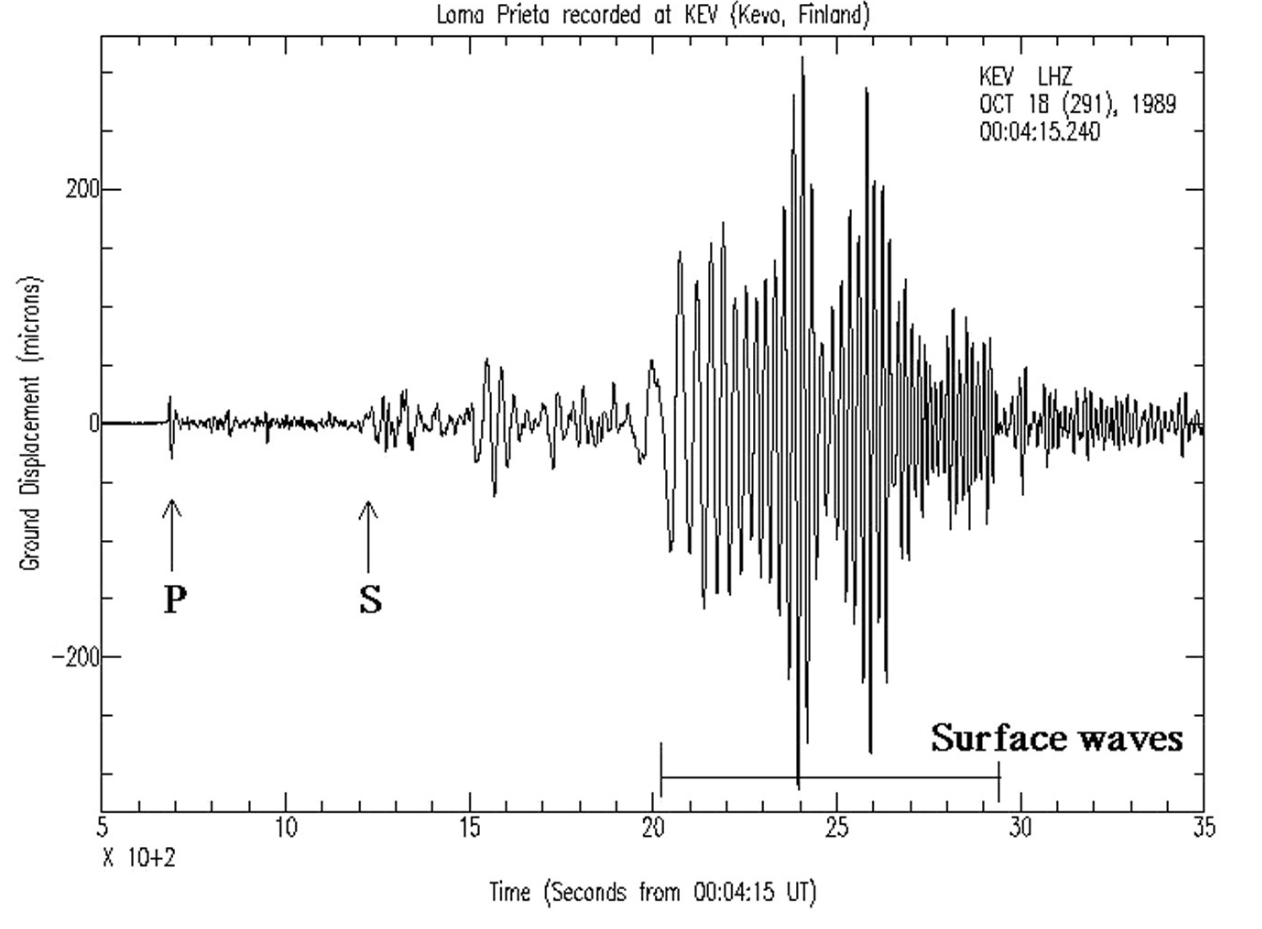
\includegraphics[width=0.8\textwidth]{figures/L6F2.png}
\caption{A vertical component seismogram recorded in Finland following an earthquake in
California. The p-wave arrival can be seen very clearly, while later arriving phases
are significantly harder to identify.}
\label{fig:fig2}
\end{figure}

The accuracy to which earthquake hypocentres can be located depends on a number of things. Clearly errors in the measured arrival times lead to uncertainties in the solution, 
but this can be assessed using standard error-propagation techniques. Next, the limited frequency content of observed seismic waves sets a fundamental limit on the accuracy of 
location estimates. If we record waves at maximum frequency of 2 Hz, then using a typical p-wave velocity of about $5 \, \text{km s}^{-1}$ for shallow parts of the Earth, we 
see that the shortest wavelengths present in the data are about 2.5 km. Such waves cannot distinguish sources separated by more than about one half or one quarter of their 
minimum wavelength\footnote{The precise fraction isn't well-defined nor is it important.}. The accuracy is also dependent on the relative locations of the seismometers to 
the source. Ideally we would like a fairly even spatial distribution in term of both azimuth and distance from the hypocentre. If, however, there are strong biases in the 
spatial distribution of the seismometers, then large uncertainties in some of the recovered parameters can be introduced. Finally, any uncertainty in the assumed Earth 
structure will clearly map onto errors in the hypocentre location. In the above discussion we have only considered the arrival times of the first waves seen on the seismograms. 
It is, however, sometimes possible to identify and measure the arrival times of other seismic phases, and these additional measurements can be used within the above procedure 
to produce better results.

\section*{The spherically averaged velocity structure of the Earth}

In the remainder of this lecture we will describe how the Earth's spherically averaged velocity has been determined using seismic observations. The basic idea behind such 
studies is very simple. After an earthquake, seismic waves propagate through the Earth's interior and are recorded at various locations around the globe. The observed 
seismograms depend on (i) the earthquake source, and (ii) the material that the waves have travelled through. And so, in principle, it is possible to work backwards from 
such observations to make inferences about both the earthquake source and the structure of the Earth's interior. Later in the course, we will see how similar ideas can 
be used to study lateral variations in the Earth's interior, this being an active area of research.

Studies of earthquake and Earth structure are fundamentally linked, and we cannot learn about one without considering the other. For example, to locate an earthquake accurately 
we must know the Earth's velocity structure, and yet these earthquake locations are required if we wish to determine the velocity structure! To proceed it is necessary to 
either consider these problems simultaneously, or to proceed in an iterative manner with one part of the problem being considered solved (i.e. that earthquake locations 
are known) while the other parameters are refined.

\subsection*{Ray theory in spherically symmetric earth models}

To learn about the Earth's velocity structure from travel time observations, we need a theory that relates these model parameters to our observations. We now show how
this can be done using asymptotic ray theory as developed in the previous lecture. For simplicity we restrict attention to isotropic earth models, in which case we need 
to consider either p-waves or s-waves, along with a whole range of converted phases that can arise at internal or external boundaries. For definiteness, we will focus 
on p-waves, but the results for s-waves or more complex phases can be handled in a similar manner.

The eikonal equation for p-waves in such a model is given by
\begin{equation}
H(\mathbf{x},\mathbf{p})=\frac{1}{2},
\end{equation}
where $\mathbf{x}$ is a position vector on a ray, $\mathbf{p}$ is the local slowness vector, and the p-wave Hamiltonian is given by
\begin{equation}
H(\mathbf{x},\mathbf{p})=\frac{1}{2}\alpha(\mathbf{x})^{2}||\mathbf{p}||^{2},
\end{equation}
with $\alpha(\mathbf{x})$ the p-wave speed at a point $\mathbf{x}$. The geometry of the ray paths is determined by solving Hamilton's canonical equations
\begin{equation}
\frac{\ddns \mathbf{x}}{\ddns \sigma}=\frac{\partial H}{\partial \mathbf{p}}, \quad \frac{\ddns \mathbf{p}}{\ddns \sigma}=-\frac{\partial H}{\partial \mathbf{x}},
\end{equation}
and the travel time $T$ along a ray is simply given by $T[\mathbf{x}(\sigma)]=\sigma$. Because the earth model under consideration is spherically symmetric, the p-wave speed 
$\alpha$ only depends on the radial distance $r=||\mathbf{x}||$ from the centre of the model. Using this fact, we will show that this problem can be solved using quadratures. 
This situation is analogous to that for a single particle in a potential, and to other "integrable systems" which having sufficiently many conserved quantities.


\begin{figure}[h]
\centering
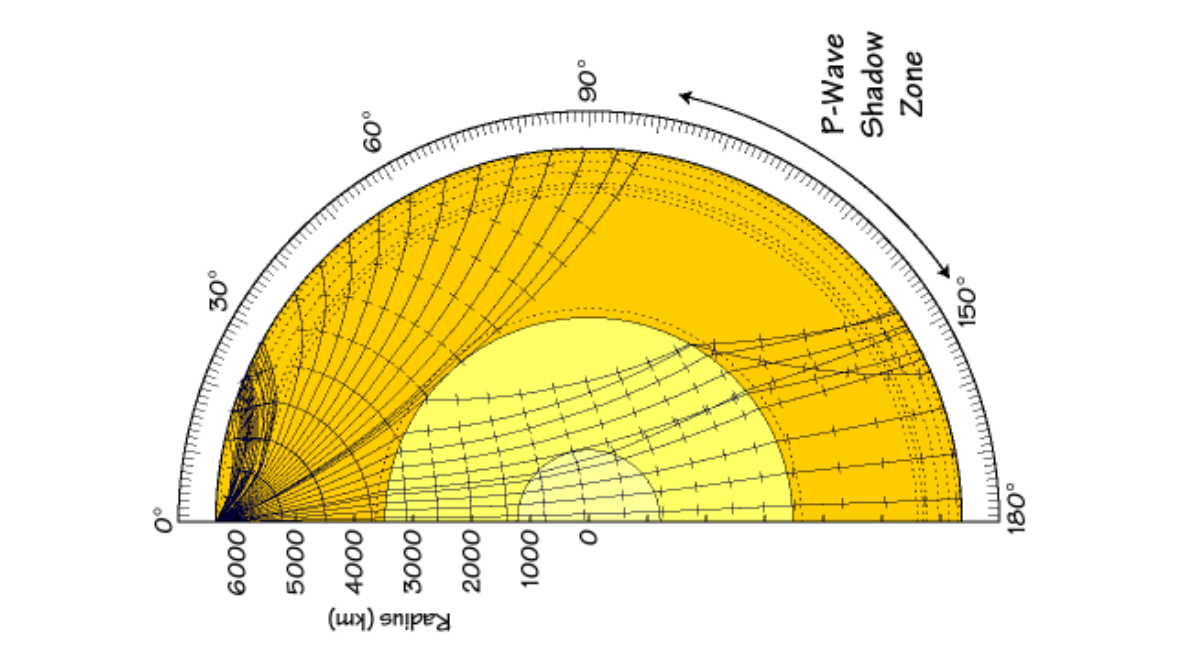
\includegraphics[width=0.8\textwidth]{figures/L6F3.png}
\caption{A diagram showing some of the many possible ray paths within the Earth. Note
in particular that the sudden reduction in p-wave velocity when entering the fluid
outer core leads to the so-called “p-wave shadow zone”, while no s-waves are able
to propagate within this region.}
\label{fig:fig3}
\end{figure}

Making use of the p-wave Hamiltonian, we find that the ray equations in eq.(5) in a spherically symmetric earth model take the specific form
\begin{equation}
\frac{\ddns \mathbf{x}}{\ddns \sigma}=\alpha\hat{\mathbf{p}}, \quad \frac{\ddns \mathbf{p}}{\ddns \sigma}=-\frac{1}{\alpha}\frac{\ddns \alpha}{\ddns r}\hat{\mathbf{x}},
\end{equation}
where we have used the eikonal equations to simplify the form of the right hand sides, and where "hats" are used to denote unit vectors. If we define $\mathbf{q}=\mathbf{x}\times \mathbf{p}$, then a simple calculation shows that
\begin{equation}
\frac{\ddns }{\ddns \sigma}(\mathbf{x}\times \mathbf{p})=\frac{\ddns \mathbf{x}}{\ddns \sigma}\times \mathbf{p}+\mathbf{x}\times\frac{\ddns \mathbf{p}}{\ddns \sigma} = \alpha\hat{\mathbf{p}}\times \mathbf{p}-\frac{1}{\alpha}\frac{\ddns \alpha}{\ddns r}\mathbf{x}\times\hat{\mathbf{x}}=0 .
\end{equation}
It follows that $\mathbf{q}$ is constant along solutions to these equations, and we mention in passing that this is precisely the conserved quantity associated with the spherical symmetry through 
Nöether's theorem. Noting from eq.(6) that $\ddns \mathbf{x}/\ddns \sigma$ is always parallel to $\mathbf{p}$, it follows that rays always remain within the plane spanned by the initial values of $\mathbf{x}$ and $\mathbf{p}$. 
Furthermore, $q=||\mathbf{q}||$ is constant along a ray, and that this can be written
\begin{equation}
q=\frac{r \sin \theta}{\alpha}
\end{equation}
where $\theta$ is the angle between $\mathbf{x}$ and $\mathbf{p}$ measured positively clockwise. Because $\mathbf{x}$ and $\mathbf{p}$ remain within their initial plane, we can write
\begin{equation}
\hat{\mathbf{p}}=\cos[\theta(\mathbf{x})]\hat{\mathbf{x}}+\sin[\theta(\mathbf{x})]\hat{\bm{\Delta}}(\mathbf{x}),
\end{equation}
where the epicentral angle $\Delta$ is that subtended between $\mathbf{x}$ and its initial value, and $\hat{\bm{\Delta}}(\mathbf{x})$ the unit vector in the direction of increasing $\Delta$ about the point $\mathbf{x}$.
Making use of eq.(8), we can then write
\begin{equation}
\sin \theta=\frac{\alpha q}{r}, \quad \cos \theta=\pm\sqrt{1-\frac{\alpha^{2}q^{2}}{r^{2}}},
\end{equation}
where the sign of the second term is determined by whether the ray is up going (+) or down going (-). For definiteness, we consider an initially down going ray, and using the first of the equations in eq.(6) we find
\begin{equation}
\frac{\ddns \mathbf{x}}{\ddns \sigma}=-\alpha\sqrt{1-\frac{\alpha^{2}q^{2}}{r^{2}}}\hat{\mathbf{x}}+\frac{\alpha^{2}q}{r}\hat{\bm{\Delta}} .
\end{equation}
In this manner, we have eliminated the local slowness vector from the problem, and are left with single equation for the position vector along the ray. To proceed, we calculate
\begin{equation}
\frac{\ddns }{\ddns \sigma}r[\mathbf{x}(\sigma)]=\frac{\partial r}{\partial x_{i}}\frac{\ddns x_{i}}{d\sigma}=-\alpha\sqrt{1-\frac{\alpha^{2}q^{2}}{r^{2}}},
\end{equation}
where we have used the familiar relation $\frac{\partial r}{\partial x_{i}}=\hat{x}_{i}$. In the same way, we find
\begin{equation}
\frac{\ddns }{\ddns \sigma}\Delta[\mathbf{x}(\sigma)]=\frac{\partial\Delta}{\partial x_{i}}\frac{\ddns x_{i}}{\ddns \sigma}=\frac{\alpha^{2}q}{r^{2}},
\end{equation}
where we have used the identity $\frac{\partial\Delta}{\partial x_{i}}=\frac{1}{r}\hat{\Delta}_{i}$ which is readily established. Combining eq.(12) and (13), we have now shown that along a ray we can write
\begin{equation}
\frac{\ddns \Delta}{\ddns r}=\frac{\ddns \Delta}{\ddns\sigma}\left(\frac{\ddns r}{\ddns \sigma}\right)^{-1}=\frac{-\alpha q}{r\sqrt{r^{2}-\alpha^{2}q^{2}}}.
\end{equation}
Similarly, using the fact that $\ddns T/\ddns \sigma=1$ along a ray, we find
\begin{equation}
\frac{\ddns T}{\ddns r}=\frac{\ddns T}{\ddns \sigma}\left(\frac{\ddns r}{\ddns \sigma}\right)^{-1}=\frac{-r}{\alpha\sqrt{r^{2}-\alpha^{2}q^{2}}}.
\end{equation}
It is important to note that these equations are only valid in portions of the ray in which the epicentral angle $\Delta$ or the travel time $T$ are single-valued functions of radius $r$.

Let us now suppose that the p-wave speed $\alpha$ increases monotonically with depth into the earth model. Consider a ray starting at the surface $r=a$ that is initially 
travelling into the earth in a non-vertical direction (i.e. $\pi/2<\theta<\pi$ initially). The fact that $q=\frac{r \sin \theta}{\alpha}$ is conserved implies that this 
ray will travel monotonically downwards into the earth with $\Delta$ monotonically increasing until it reaches a turning point $r_{t}$ such that
\begin{equation}
q=\frac{r_{t}}{\alpha(r_{t})}
\end{equation}
Beyond this turning point, the ray moves up towards the surface, with r monotonically increasing, and $\Delta$ continuing to monotonically increase. Furthermore, the up and down 
going legs of the rays path are symmetric about the radial line passing through the turning point. Using eq.(14) which is valid throughout the down going leg, we obtain
\begin{equation}
\Delta=\int_{r_{t}}^{a}\frac{2\alpha(r)q}{r\sqrt{r^{2}-\alpha(r)^{2}q^{2}}}\dd r;
\end{equation}
for the total epicentral angle subtended by the ray as it travels from the surface to the turning point and then up to the surface again. Using eq.(15) we similarly write the travel time along this ray path as
\begin{equation}
T=\int_{r_{t}}^{a}\frac{2r}{\alpha(r)\sqrt{r^{2}-\alpha(r)^{2}q^{2}}}\dd r.
\end{equation}
In this manner, we see that the travel time along a ray path in such a spherical model can be obtained through a simple integral over the velocity structure (the integrands are 
singular at the turning points, but these are integrable singularities). The extension of these results to models having more complicated velocity structures is 
straightforward in principle, but takes a little effort.

\subsection*{Travel time inversions for spherical velocity structure}
As we have just seen, ray theory can be used to efficiently determine the travel times of various seismic phases within a spherically symmetric earth model. At a given epicentral 
angle, there will generally be many distinct seismic phases that arrive at different times and correspond to different ray paths as well as non-geometric phases such as surface 
waves, head waves, and diffracted waves that are not predicted by ray theory. The use of the word ``phase'' here refers to a distinct waveform on a seismogram, and should not 
be confused with other uses of ``phase'' within these lectures or elsewhere.

Assuming that we know an earthquake's location and origin time, it is possible to measure the travel times of various seismic phases to different seismometers. By repeating 
this process for many many events, global averaged travel time curves have been constructed. Given a radial velocity structure, we know how to calculate travel times for 
the different phases, and we aim to find an earth model that is consistent with our observations. This is another example of an inverse problem in which we must work 
backwards from observations to learn about a set of model parameters. We will have more to say about inverse problems later in the course, but historically speaking, 
the determination of the Earth's spherically symmetric velocity structure largely pre-dates the introduction of inverse theory, and early studies used more-or-less ad 
hoc methods. In this field, the most important figures are Richard Oldham (1858-1936), Beno Gutenberg (1889-1960), Harold Jeffreys (1891-1989), and 
Inge Lehmann (1888-1993). In particular, it was Oldham who first identified the Earth's core by noting the absence of p-wave arrivals within a certain range of 
epicentral angles. Jeffreys first convincingly argued that the core of the Earth must be at least partially fluid, though here the relevant observations were 
of solid-Earth tides, and not seismic waves. Finally, Lehmann later realised that there exists a solid inner core through careful study of waves travelling 
through the Earth's central region. There is a famous quote from Oldham's 1906 paper on the Earth's core that is worth repeating:
\begin{quote}
``Of all regions of the Earth none invites speculation more than that which lies beneath our feet, and in none is speculation more dangerous; yet, apart from 
speculation, it is little that we can say regarding the constitution of the interior of the earth. Many theories of the earth have been propounded at different 
times: the central substance of the earth has been supposed to be fiery, fluid, solid, and gaseous in turn, till geologists have turned in despair from the 
subject, and become inclined to confine their attention to the outermost crust of the Earth, leaving its centre as a playground for mathematicians.''
\end{quote}
We shall not consider the determination of the spherically symmetric velocity structure further, but will instead turn to discussing the broad features that have been learnt about the spherically symmetric velocity structure.

\subsection*{An overview of the Earth's spherically averaged velocity structure}


\begin{figure}[h]
\centering
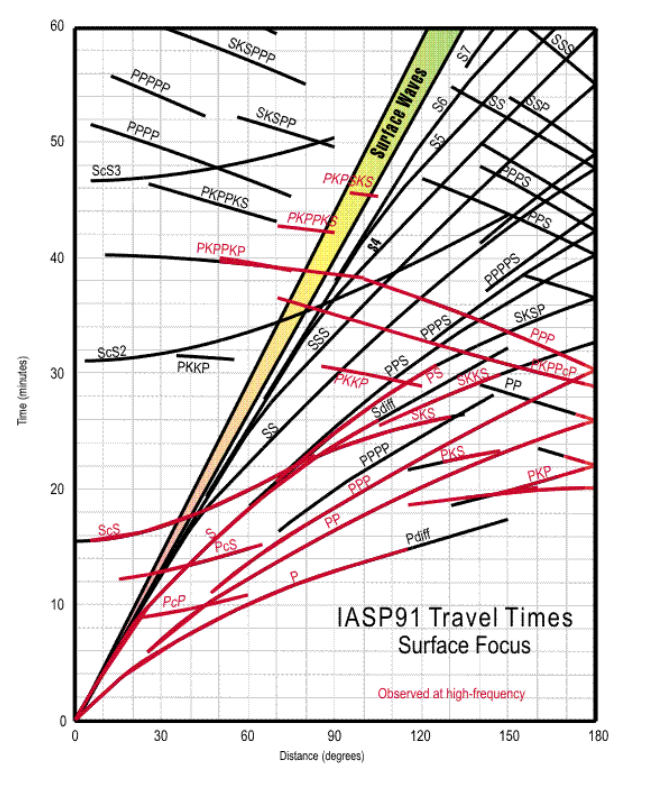
\includegraphics[width=0.8\textwidth]{figures/L6F4.png}
\caption{Travel time curves determined for a large number of seismic phases within the
Earth. The nomenclature for the different phases can be ignored.}
\label{fig:fig4}
\end{figure}

The model PREM by Dziewonski \& Anderson (1981) shows the variation of p-wave and s-wave velocity with depth in the earth. This model was obtained by fitting travel 
times of seismic waves, as well as further constraints obtained from observations of the Earth's free oscillations that will be the focus of a later lecture. As a 
first observation, there is a a general tendency for the velocity to increase gradually downwards, though there are also a number of sharp discontinuities within 
the structure. The p-wave velocity $\alpha$ and s-wave velocity $\beta$ are given by
\begin{equation}
\alpha=\sqrt{\frac{\kappa+\frac{4}{3}\mu}{\rho}}, \quad \beta=\sqrt{\frac{\mu}{\rho}},
\end{equation}
where $\kappa$ is the bulk modulus, $\mu$ the shear modulus, and $\rho$ the density. As we go deeper into the Earth, things are increasingly compressed, and this tends to 
increase both the elastic modulii and the density, though the combined effect is typically for wave velocities to increase.

Discontinuities in the seismic velocity are identified principally by the occurrence of reflected seismic waves, and their presence must be due to sharp changes in either 
the composition or through a phase change within the same material. Note here that ``sharp'' is always defined relative to the wavelength of the seismic waves used to image 
the Earth, and so these boundaries may, in reality, be somewhat diffuse. The most notable discontinuities within the Earth are at the core mantle boundary (CMB) which is 
thought to represent a change from the rocky mantle to a fluid iron core, and at the inner core boundary (ICB) which is explained by a fluid to solid phase change within 
the iron core. It is worth emphasising that we do not actually know that the core is made of iron (and likely a few additional minor components). The reasons for thinking 
this is likely are: (i) iron at the appropriate pressures and temperatures has the right sort of density and wave speeds, (ii) iron is very abundant in the solar system due 
to its high binding energy, (iii) there exist iron meteorites that are interpreted as fragments from the cores of ``proto-planets'', and (iv) such a composition is consistent 
with the generation of the geodynamo in a convecting conductor.


\begin{figure}[h]
\centering
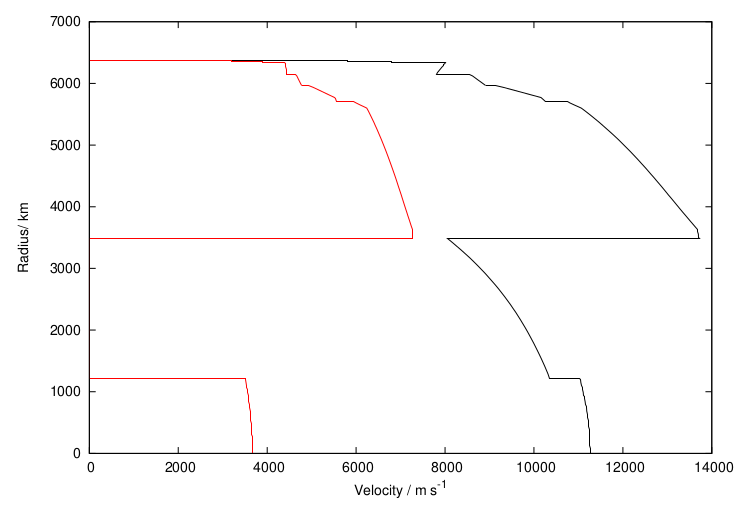
\includegraphics[width=0.8\textwidth]{figures/L6F5.png}
\caption{Variation of p-wave velocity (black curve) and s-wave velocity (red curve) with
radius in the model PREM of Dziewonski \& Anderson (1981). Here we can see that
both wave speeds generally increase with depth, but this increase is interrupted by
a number of sharp velocity discontinuities. Such discontinuities are associated with
compositional or phase changes within the Earth. The most notable boundaries
within the Earth are between the the rocky mantle and the fluid iron outer core
where the s-wave velocity becomes equal to zero, and at the inner core boundary
where the iron of the core undergoes a fluid to solid phase transformation.}
\label{fig:fig5}
\end{figure}

That the outer core is a fluid is strongly suggested by (i) observations of solid-Earth tides, (ii) the absence of s-waves propagating through this region ($\mu=0$ in a fluid), 
and (iii) is also required for the generation of the geodynamo. The likely solidity of the inner core has been deduced by a number of arguments. Firstly, it does not seem plausible 
that there could be a sharp jump in velocity within a purely fluid region. There is also compelling evidence derived from the observed free oscillation periods (Dziewonski \& 
Gilbert 1975). And lastly, some studies that have identify inner core s-waves produced by conversion from a p-wave at the ICB (e.g. Deuss et al. 2000). Such core phases have 
very small amplitudes and the robustness of such observations are still debated.

As well as the velocity discontinuities at the CMB and ICB, there are a number of other discontinuities within the shallower Earth. Those within the crust and upper most mantle 
are almost certainly due to compositional changes. There are then additional discontinuities at around 410 km and 670 km that are not readily explained in terms of composition. 
Instead these discontinuities are thought to represent solid-state phase transformations within the minerals making up the Earth's mantle that result from radial changes in both 
pressure and temperature. The occurrence of such phase transformations within this part of the mantle is consistent with both laboratory experiments and quantum mechanical calculations. 
The region between the 410 km and 670 km discontinuities is known as the transition zone, and can be regarded as separating the upper and lower parts of the mantle. Other 
properties such as viscosity are believed to also be discontinuous across these phase boundaries, with the lower mantle seeming to be significantly more viscous. The 
viscosity contrast between the upper and lower mantle has important implications for mantle convection, and may lead to some "decoupling" of the two regions.

\section*{What you need to know and be able to do}
\begin{itemize}
    \item[(i)] Know what the hypocentre of an earthquake is, and how the hypocentral location and time can be determined using observations of seismic waves.
    \item[(ii)] Understand how the Hamiltonian ray tracing equations within a spherically symmetric earth model can be reduced to the calculation of 
    appropriate radial integrals. Within the second problem set, you will work through similar calculations in a horizontally stratified earth model.
    \item[(iii)] Understand in outline the observations and methods that were used to constrain the Earth's spherically symmetric velocity structure. 
    You should also know the basic properties of this spherically symmetric velocity structure, and the physical interpretation of its major features.
\end{itemize}

\end{document}
